\documentclass[9pt,aspectratio=169]{beamer}

%============================================================
% THEME AND PACKAGES
%============================================================
\usetheme{Madrid}
\usefonttheme{professionalfonts}

\usepackage{amsmath,amssymb,mathtools}
\usepackage{booktabs,array}
\usepackage{tikz}
\usetikzlibrary{arrows.meta,positioning,calc,fit}

%============================================================
% COLOUR THEME
%============================================================
\definecolor{accent}{RGB}{42,86,82}
\definecolor{accentlight}{RGB}{232,241,239}
\definecolor{slate}{RGB}{61,70,77}
\definecolor{softgray}{RGB}{246,247,247}

\setbeamercolor{structure}{fg=accent}
\setbeamercolor{frametitle}{fg=accent,bg=white}
\setbeamercolor{title}{fg=accent}
\setbeamercolor{block title}{fg=accent,bg=accentlight}
\setbeamercolor{block body}{fg=black,bg=softgray}
\setbeamercolor{block title alerted}{fg=white,bg=slate}
\setbeamercolor{block body alerted}{fg=black,bg=softgray}

\setbeamerfont{block title}{size=\small}
\setbeamertemplate{navigation symbols}{}
\setbeamertemplate{itemize item}
    {\color{accent}\scriptsize$\blacktriangleright$}

\setbeamersize{text margin left=5mm,text margin right=5mm}

\setlength{\abovedisplayskip}{3pt}
\setlength{\belowdisplayskip}{3pt}
\setlength{\abovedisplayshortskip}{2pt}
\setlength{\belowdisplayshortskip}{2pt}

%============================================================
% TITLE AND HELPERS
%============================================================
\title{Stealthy Computational Delay Attacks on Control Systems}
\subtitle{Project Introduction: System Model, Attack Optimization, and Detection}
\author{}
\date{}

\newcommand{\paperref}{\tiny Source: T. Nauta, H. Sandberg, and M. Maggio, ``Stealthy Computational Delay Attacks on Control Systems,'' ICCPS 2025.}

\newcommand{\tightitemize}{
    \setlength{\itemsep}{1.5pt}
    \setlength{\parskip}{0pt}
    \setlength{\topsep}{2pt}
}

\begin{document}

%============================================================
% SLIDE 1 — MOTIVATION
%============================================================
\begin{frame}{Motivation: Why Computational-Delay Attacks?}

\begin{columns}[T,onlytextwidth]

\begin{column}{0.53\textwidth}

\begin{block}{Attack scenario}
\begin{itemize}
\tightitemize
    \item A real-time controller must finish each control
    computation before its deadline.

    \item An attacker can cause \textbf{CPU starvation or
    execution delays}, making a control job miss its deadline.

    \item The attacker need not alter the sensor measurement
    or plant equations. The physical plant may be harmed
    because a fresh control command is unavailable on time.
\end{itemize}
\end{block}

\begin{alertblock}{Research question}
\centering
\textbf{How can an attacker maximize physical disruption
while avoiding timing-based detection?}
\end{alertblock}

\end{column}

\begin{column}{0.45\textwidth}

\begin{block}{Closed-loop attack path}
\centering

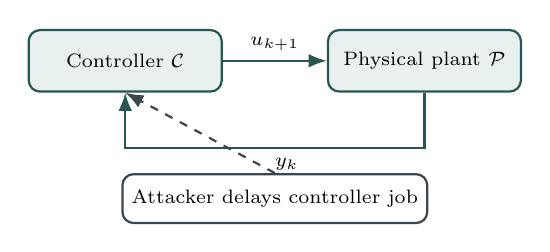
\begin{tikzpicture}[
    >=Latex,
    every node/.style={font=\scriptsize},
    blk/.style={
        draw=accent,
        fill=accentlight,
        rounded corners,
        thick,
        align=center,
        minimum width=2.45cm,
        minimum height=0.78cm
    },
    atk/.style={
        draw=slate,
        fill=white,
        rounded corners,
        thick,
        align=center,
        minimum width=2.45cm,
        minimum height=0.62cm
    },
    arr/.style={->,thick,draw=accent}
]

\node[blk] (c) at (0,1.9)
    {Controller $\mathcal C$};

\node[blk] (p) at (3.8,1.9)
    {Physical plant $\mathcal P$};

% Forward control path
\draw[arr] (c.east)
    -- node[above] {$u_{k+1}$} (p.west);

% Feedback path
\draw[arr] (p.south)
    -- ++(0,-0.70)
    -| node[pos=0.23,below] {$y_k$} (c.south);

% Attacker
\node[atk] (a) at (1.9,0.15)
    {Attacker delays controller job};

\draw[->,thick,dashed,draw=slate]
    (a.north) -- (c.south);

\end{tikzpicture}

\vspace{1mm}

\small The plant continues evolving even when the controller
misses a deadline.

\end{block}

\begin{block}{Separate the contributions}
\begin{itemize}
\tightitemize
    \item \textbf{Paper:} attack model, optimization formulation,
    and statistical detector analysis.

    \item \textbf{This project:} physical/interactive demonstration
    and analysis of defender parameters.
\end{itemize}
\end{block}

\end{column}
\end{columns}

\vfill
{\paperref}

\end{frame}


%============================================================
% SLIDE 2 — PLANT AND CONTROLLER
%============================================================
\begin{frame}{Discrete-Time Plant and Controller}

\begin{columns}[T,onlytextwidth]

\begin{column}{0.49\textwidth}

\begin{block}{Physical plant --- Eq. (1)}

\[
\boxed{
\begin{aligned}
x_{k+1}&=Ax_k+Bu_k,\\
y_k&=Cx_k+Du_k.
\end{aligned}
}
\]

\vspace{-1mm}

\begin{itemize}
\tightitemize
    \item $x_k$: plant state
    \item $u_k$: applied plant input
    \item $y_k$: plant output/measurement
\end{itemize}

\end{block}

\begin{block}{Controller --- Eq. (2)}

\[
\boxed{
\begin{aligned}
z_{k+1}&=Fz_k+Gy_k,\\
u_{k+1}&=Hz_k+Ky_k.
\end{aligned}
}
\]

\vspace{-1mm}

\begin{itemize}
\tightitemize
    \item $z_k$: controller state
    \item $y_k$: measured plant output
    \item $u_{k+1}$: command for the next period
\end{itemize}

\end{block}

\end{column}


\begin{column}{0.49\textwidth}

\begin{block}{Complete physical feedback loop}
\centering

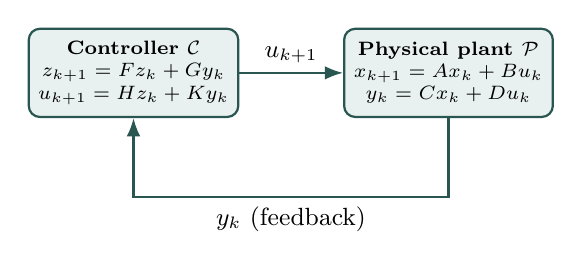
\begin{tikzpicture}[
    >=Latex,
    blk/.style={
        draw=accent,
        fill=accentlight,
        rounded corners,
        thick,
        minimum width=2.65cm,
        minimum height=1.12cm,
        align=center,
        font=\scriptsize
    },
    sig/.style={->,thick,draw=accent}
]

\node[blk] (c) at (0,1.65)
{
    \textbf{Controller $\mathcal C$}\\
    $z_{k+1}=Fz_k+Gy_k$\\
    $u_{k+1}=Hz_k+Ky_k$
};

\node[blk] (p) at (4.0,1.65)
{
    \textbf{Physical plant $\mathcal P$}\\
    $x_{k+1}=Ax_k+Bu_k$\\
    $y_k=Cx_k+Du_k$
};

% Controller to plant
\draw[sig] (c.east)
    -- node[above,font=\small] {$u_{k+1}$} (p.west);

% Plant feedback to controller
\draw[sig] (p.south)
    -- ++(0,-1.0)
    -| node[pos=0.25,below,font=\small] {$y_k$ (feedback)}
    (c.south);

\end{tikzpicture}

\end{block}

\begin{alertblock}{Timing convention}
\footnotesize
During period $k$, the plant holds $u_k$ constant. The
controller measures $y_k$ and computes $u_{k+1}$ for period
$k+1$. The nominal control objective is to regulate the
output toward zero.
\end{alertblock}

\end{column}
\end{columns}

\vfill
{\paperref}

\end{frame}


%============================================================
% SLIDE 3 — DELAY ATTACK AND SWITCHED DYNAMICS
%============================================================
\begin{frame}{Computational Delay Attack and Switched Dynamics}

\footnotesize

\begin{columns}[T,onlytextwidth]

\begin{column}{0.51\textwidth}

\begin{block}{Augmented closed-loop state}

The state includes the plant, controller, and stored information:

\[
\boxed{
\psi_k=
\begin{bmatrix}
x_k\\
\tilde y_k\\
z_k\\
u_k
\end{bmatrix}
}
\]

\vspace{-1mm}

\scriptsize
$\tilde y_k$ is the latest stored measurement.
The augmented state $\psi_k$ captures the complete
closed-loop state used by the attack model.

\end{block}

\begin{block}{Binary deadline decision}

\[
a_k=
\begin{cases}
0,&\text{deadline hit},\\
1,&\text{deadline miss}.
\end{cases}
\]

\[
\boxed{
\psi_{k+1}
=
\big[(1-a_k)\Phi_h+a_k\Phi_m\big]\psi_k
}
\]

\scriptsize
$\Phi_h$ and $\Phi_m$ are the hit- and miss-mode matrices
(paper's switched model, Eq. (7)).

\end{block}

\end{column}


\begin{column}{0.47\textwidth}

\begin{block}{What happens on a missed deadline?}

\begin{itemize}
\tightitemize
    \item The physical plant continues evolving.
    \item Controller computation is delayed; the controller
    state and stored measurement are not updated.
    \item The actuator either \textbf{HOLDs} the previous
    command or applies \textbf{ZERO}.
\end{itemize}

\end{block}


\begin{block}{Example sequence: $11010$}
\centering

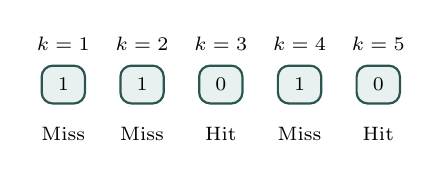
\begin{tikzpicture}[
    every node/.style={font=\scriptsize},
    bit/.style={
        draw=accent,
        rounded corners,
        minimum width=0.55cm,
        minimum height=0.48cm,
        thick,
        fill=accentlight
    },
    status/.style={align=center,minimum width=0.68cm}
]

\foreach \x/\b/\s/\k in
    {0/1/Miss/1,1.0/1/Miss/2,2.0/0/Hit/3,
     3.0/1/Miss/4,4.0/0/Hit/5}
{
    \node[bit] at (\x,0.2) {\b};
    \node[status] at (\x,-0.43) {\s};
    \node[status] at (\x,0.72) {$k=\k$};
}

\end{tikzpicture}

\vspace{1mm}

\scriptsize
$1$ = miss; $0$ = hit. The attacker chooses timing failures,
not the output directly.

\end{block}

\end{column}
\end{columns}

\vfill
{\paperref}

\end{frame}


%============================================================
% SLIDE 4 — OPTIMIZATION AND ATTACK EFFECTIVENESS
%============================================================
\begin{frame}{Optimal Stealthy Attack: Impact Under Constraints}

\begin{columns}[T,onlytextwidth]

\begin{column}{0.61\textwidth}

\begin{block}{Compact optimization formulation}

\small

\[
\begin{aligned}
\max_{a_0,\ldots,a_{\ell-1}}\quad
    &y_\ell^{\mathsf T}Qy_\ell\\[-1mm]
\text{subject to}\quad
    &a_k\in\{0,1\},
      \quad k=0,\ldots,\ell-1,\\[-1mm]
    &\sum_{q=j}^{j+\bar a}a_q\leq\bar a,\\
    &\hspace{5mm}j=0,\ldots,\ell-\bar a-1,\\[-1mm]
    &\psi_{k+1}
      =\big[(1-a_k)\Phi_h+a_k\Phi_m\big]\psi_k,\\[-1mm]
    &\text{binomial and geometric stealth constraints.}
\end{aligned}
\]

\end{block}

\begin{itemize}
\tightitemize
    \item $a_k$: binary attack decisions; $\ell$: attack horizon.
    \item The watchdog constraint limits consecutive misses.
    \item Gurobi optimizes the feasible miss sequence; it does
    not choose $Q$ or directly set $y_\ell$.
\end{itemize}

\end{column}


\begin{column}{0.37\textwidth}

\begin{block}{Do not conflate these quantities}

\[
J_{\mathrm{attack}}(\ell)
=y_\ell^{\mathsf T}Qy_\ell
\]

\[
\boxed{
\omega(\ell)
=
J_{\mathrm{attack}}(\ell)
-
J_{\mathrm{nominal}}(\ell)
}
\]

\small
Both trajectories start from the same initial conditions.
The objective is the quantity maximized; $\omega(\ell)$
measures the additional deviation relative to the
no-attack baseline.

\end{block}

\begin{block}{Output weighting $Q$}

\scriptsize

\begin{itemize}
\tightitemize
    \item Furuta pendulum:
    $Q=\operatorname{diag}(1,0,0)$
    (pendulum angle).

    \item Quadruple tank:
    $Q=\operatorname{diag}(1,1)$
    (both regulated outputs).
\end{itemize}

$Q=I$ is a mathematical illustration, not a universal choice.

\end{block}

\end{column}
\end{columns}

\vfill
{\paperref}

\end{frame}


%============================================================
% SLIDE 5 — WATCHDOG AND BINOMIAL DETECTOR
%============================================================
\begin{frame}{Detection I: Watchdog and Binomial Test}

\footnotesize

\begin{columns}[T,onlytextwidth]

\begin{column}{0.40\textwidth}

\begin{block}{Watchdog: consecutive misses}

\[
\boxed{
\text{No more than }\bar a
\text{ consecutive misses}
}
\]

\begin{itemize}
\tightitemize
    \item $a_k=1$ denotes a deadline miss.
    \item If $\bar a=2$, three consecutive misses violate
    the watchdog rule.
    \item Passing the watchdog limits runs, but not necessarily
    the total number of misses in a window.
\end{itemize}

\end{block}

\begin{block}{Model assumption}

\scriptsize
Nominal misses are modeled as independent events with
estimated probability $\hat p_m$. This is an assumption,
not a universal property of every real-time system.
\end{block}

\end{column}


\begin{column}{0.58\textwidth}

\begin{block}{Sliding-window binomial test}

Let $w_i\in\{0,1\}$ denote the hit/miss status of job $i$
in a window of $n_w$ jobs, where $1$ denotes a miss.

\[
S_w=\sum_{i=1}^{n_w}w_i
\]

Under the nominal model,

\[
S_w\sim\operatorname{Binomial}(n_w,\hat p_m).
\]

The one-sided hypotheses are

\[
H_0:p\leq\hat p_m,
\qquad
H_1:p>\hat p_m.
\]

The sequence passes the binomial test when

\[
\boxed{
\sum_{i=1}^{n_w}w_i
\leq
\mathcal B_{1-\alpha}(n_w,\hat p_m)
}
\]

\scriptsize
$\mathcal B_{1-\alpha}$ is the binomial critical count;
$\alpha$ is the significance level.

\end{block}

\end{column}
\end{columns}

\vspace{1mm}

{\scriptsize
\textbf{Key distinction:} the watchdog limits consecutive
misses; the binomial test limits the total miss count in a
window. Passing a test does not prove that no attack is present.
}

\vfill
{\paperref}

\end{frame}


%============================================================
% SLIDE 6 — GEOMETRIC AND CHI-SQUARE DETECTOR
%============================================================
\begin{frame}{Detection II: Geometric Run-Length and $\chi^2$ Test}

\footnotesize

\begin{columns}[T,onlytextwidth]

\begin{column}{0.51\textwidth}

\begin{block}{Run-length categories}

Let $R$ be the number of consecutive misses before a hit.
The final category groups the tail at the watchdog limit:

\[
P(R=r)=
\begin{cases}
\hat p_m^{\,r}(1-\hat p_m),
    &0\leq r<\bar a,\\[1mm]
\hat p_m^{\,\bar a},
    &r=\bar a.
\end{cases}
\]

\scriptsize
The categories are $r=0,1,\ldots,\bar a$; the final
category groups the tail run length.

\end{block}

\begin{block}{Expected and observed counts}

If $N$ is the total number of completed jobs used in
the geometric test, then

\[
\boxed{
E_r=NP(R=r)
}
\]

where $m_r$ is the observed count for category $r$.

\end{block}

\end{column}


\begin{column}{0.47\textwidth}

\begin{block}{Chi-square statistic}

\[
\boxed{
S_{\chi^2}
=
\sum_{r=0}^{\bar a}
\frac{(m_r-E_r)^2}{E_r}
}
\]

The acceptance condition is

\[
\boxed{
S_{\chi^2}
\leq
\chi^2_{1-\alpha}(\bar a)
}
\]

\scriptsize
$\chi^2_{1-\alpha}(\bar a)$ is the critical value at
significance level $\alpha$, using the paper's
degrees of freedom.

\end{block}

\begin{alertblock}{Why use both statistical tests?}

\scriptsize
A sequence may satisfy the watchdog yet have an abnormal
run-length pattern. The binomial test checks miss counts;
the geometric/$\chi^2$ test checks run-length frequencies.

\end{alertblock}

\end{column}
\end{columns}

\vfill
{\paperref}

\end{frame}

\end{document}